\documentclass[prb,showpacs,floatfix,altaffilletter,amsmath,amssymb,reprint,citeautoscript]{revtex4-1}
\usepackage{custom}
\usepackage{chng}

\begin{document}

\title{Amplificatore lock-in ad allineamento in fase per la misura dei coefficienti di Fresnel su cristalli non dielettrici}
\author{Mattia Sotgia}
\email{s4942225@studenti.unige.it}
\author{Francesco Polleri}
\email{s5025011@studenti.unige.it}
\affiliation{Università degli Studi di Genova, Dipartimento di Fisica}
\date{\today}

\begin{abstract}
    Presentiamo la progettazione e la realizzazione di un esperimento per la misura dei coefficienti di Fresnel di un film sottile di cristallo di Silicio (c-Si) e su un sottile campione di oro (Au). La misura è effettuata sfruttando un sistema di accoppiamento di fase lock-in\cite{scofieldFrequencydomainDescriptionLockin1994} che permette una migliore reiezione in frequenza del rumore. Descriviamo la progettazione del sistema di misura, e infine una descrizione e discussione dei risultati, confrontando con modelli teorici. Il sistema descritto permette di effettuare misure con sufficiente precisione dei coefficienti di Fresnel $R_s$ e $R_p$, permettendo di ottenere i coefficienti di riflessione e trasporto $n_\text{c-Si}/k_\text{c-Si}$ e $n_\text{Au}/n_\text{Au}$. Per il cristallo di silicio (c-Si) possiamo anche inferire il valore dello spessore del film di ossido di silicio ($\mathrm{SiO_2}$) depositato sul substrato di silicio.
    %\comment{Aggiungere anche alcuni commenti riguardo ai risultati ottenuti}
\end{abstract}
\maketitle

\section{Introduzione} 

L'utilizzo di un sistema sensibile allo sfasamento, come un amplificatore lock-in, può risultare molto comodo in applicazioni di misura in cui si fa utilizzo di segnali luminosi. In questo modo è infatti possibile ridurre sufficientemente i disturbi e le interferenze prodotte dal rumore esterno, che in un ambiente di laboratorio possono essere molteplici, e inoltre permette anche di controllare e ridurre anche fonti di rumore che sono invece causate dal sistema stesso, come possono essere problemi di surriscaldamento e quindi variazione dell'intensità di emissione del fotodiodo, oppure effetti di carattere aleatorio in acquisizione del fototransitor. Considerando allora un sistema che permette di generare e di acquisire con una fase definita, possiamo infatti ridurre molti di questi contributi di rumore, e quindi incrementare il rapporto tra segnale e rumore (SNR). 


\paragraph*{Teoria}\begin{equation}
    r_\mathrm{p} = \frac{\Tilde{n}_2\cos\theta_i - \Tilde{n}_1\cos\theta_t}{\Tilde{n}_2\cos\theta_i + \Tilde{n}_1\cos\theta_t}
\end{equation}
\begin{equation}
    r_\mathrm{s} = \frac{\Tilde{n}_1\cos\theta_i - \Tilde{n}_2\cos\theta_t}{\Tilde{n}_1\cos\theta_i + \Tilde{n}_2\cos\theta_t}
\end{equation}
\begin{equation}
    \cos\theta_t = \sqrt{1-\qty(\frac{\Tilde n_1}{\Tilde n_2}\sin\theta_i)^2}
\end{equation}

\section{Metodi}

\paragraph*{L'esperimento} 
L'esperimento è definito da una sorgente di luce coerente debolmente polarizzata, trasmessa e incidente \replace[FP]{sul bersaglio semitrasparente, e il segnale riflesso è in linea con il rivelatore che permette di misurare l'intensità del fascio incidente.È possibile interporre sul cammino ottico del fascio laser un rivelatore di intensità luminosa, ovvero un fototransistor, e delle lenti polarizzatrici.}{su un bersaglio semitrasparente che genera un fascio riflesso che è in linea con un rivelatore di intensità luminosa costituito da un fototransistor. Sul cammino ottico di questo fascio è inoltre possibile inserire delle lenti polarizzatrici.}

Il segnale luminoso è prodotto da una sorgente coerente \comment[MS]{Dobbiamo descrivere accuratamente le caratteristiche del laser utilizzato.} verde, controllato da un segnale periodico che ne permette l'accoppiamento in fase con il ricevitore.\comment[FP]{Parliamo qui del chopper o dopo?} In questo modo possiamo ridurre gli effetti aleatori legati alla produzione e alla ricezione del segnale fisico. Il segnale luminoso è quindi fatto passare in aria e attraverso \replace[FP]{un primo filtro polarizzatore: l'inserimento di questa componente ottica permette di controllare l'angolo con cui la radiazione incidente è polarizzato.}{due filtri polarizzatori. Il primo filtro serve per controllare l'intensità del fascio (vedi legge di Malus) mentre il secondo filtro ci dà la polarizzazione finale con cui il fascio incide sul campione.} Infatti il laser produce un segnale coerente che dovrebbe essere idealmente non polarizzato, ma che realmente \replace[FP]{è invece polarizzato.}{invece lo è almeno in parte} L'angolo di polarizzazione viene misurato in relazione alla superficie dell'interfaccia riflettente del campione, che è presa come zero, nella direzione verso l'alto. La normale esterna al campione è presa quindi come massimo per il $\cos\theta$, per cui $\theta = \SI{90}{\degree}$. 

\begin{figure}
    \centering
    \subfloat{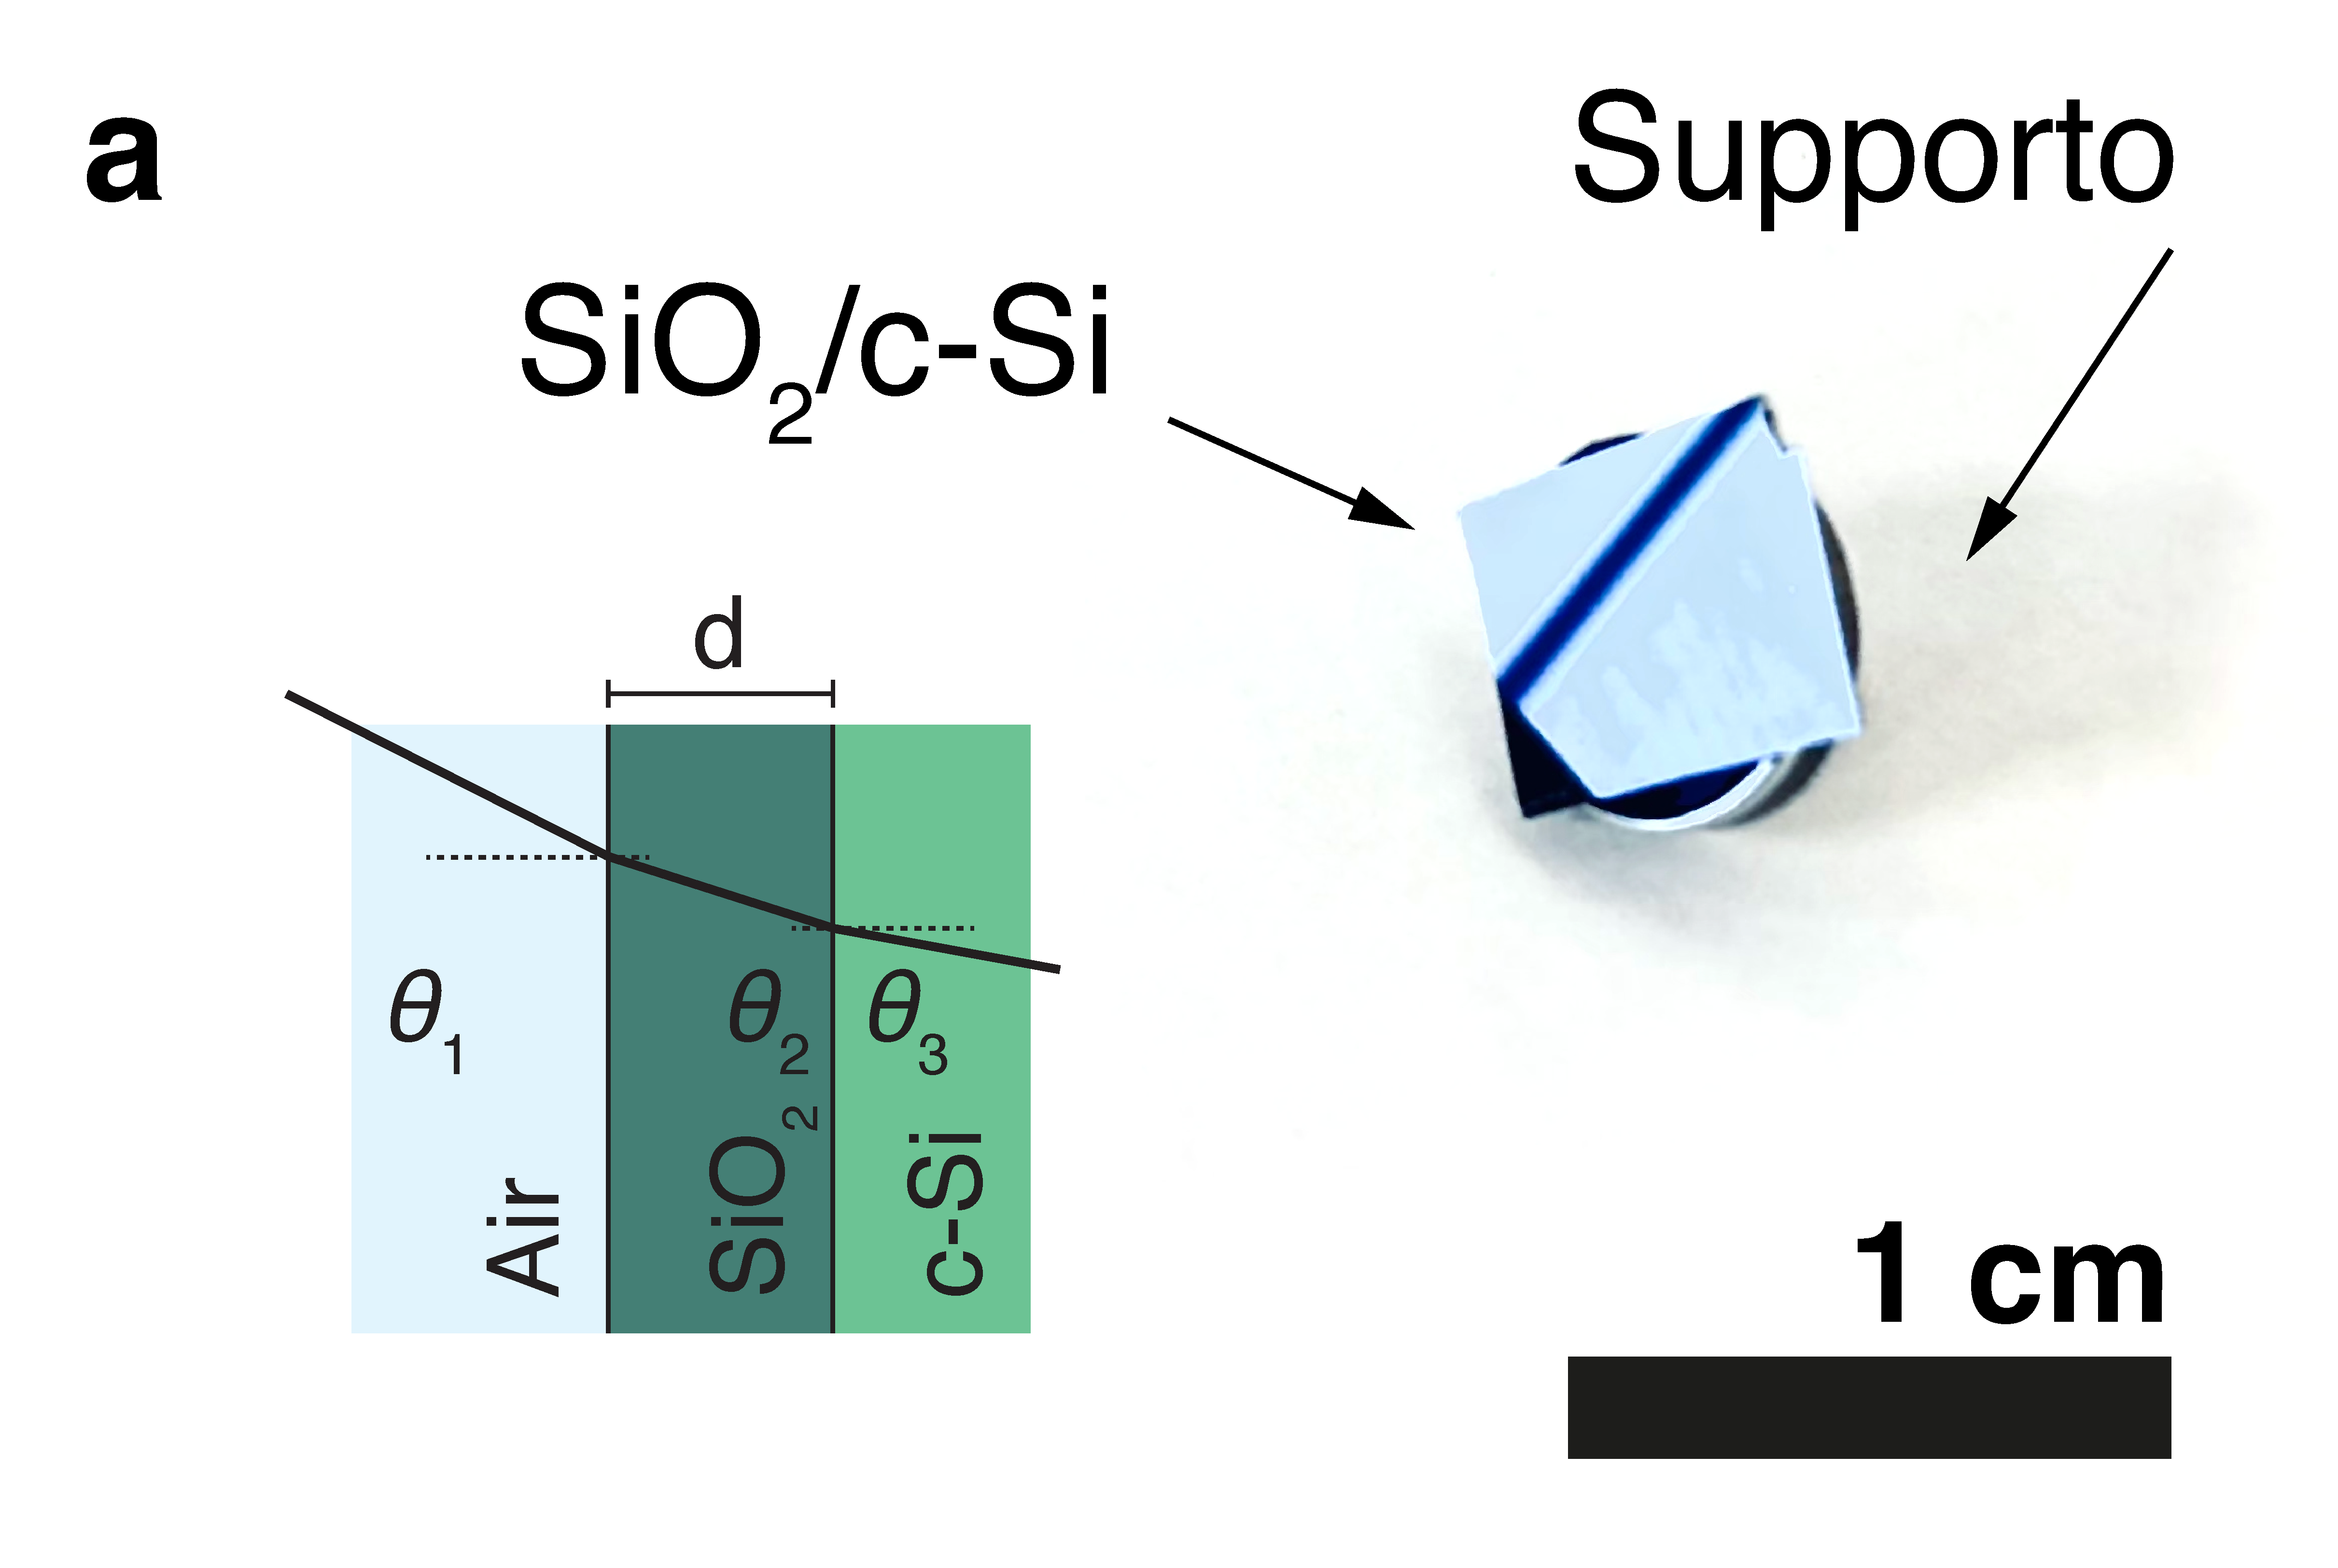
\includegraphics[width=\linewidth,trim={0 4cm 0 0}]{figures/c-Si.pdf}\label{fig:c-Si}}
    
    \subfloat{\includegraphics[width=\linewidth]{figures/Au_sample.pdf}\label{fig:Au}}
    \caption{\ref{sub@fig:c-Si} Campione di  cristallo di Silicio montato sul supporto necessario per poter effettuare le misure. A lato è anche schematizzata la struttura a layer dell'interfaccia del c-Si con l'aria, a cui è interposto un sottile strato di $\mathrm{SiO_2}$ che cambia quindi l'angolo con cui la luce incide sul silicio. \ref{sub@fig:Au} Campione di oro e schema della struttura dell'interfaccia aria/oro. }
\end{figure}

\begin{figure}
    \centering
    \includegraphics[width=\linewidth,trim={0 8cm 0 0}]{figures/photoDiode.pdf}
    \caption{Immagine del fotodiodo utilizzato per la acquisizione dei dati. Il laser colpisce ortogonalmente il cristallo semiconduttore , che ha una apertura angolare di circa \SI{2}{\degree}, sulla quale la risposta è pressoché uniforme, come possiamo dedurre anche dal grafico, ad eccezione fatta per le regioni ai bordi, evidenziate in verde, per le quali interviene il fattore di forma del fascio di luce laser, che per quanto estremamente collimato presenta una distribuzione approssimativamente gaussiana, della quale stiamo osservando le code. }
    \label{fig:photo-diode}
\end{figure}

\begin{figure*}
    \centering
    \subfloat[]{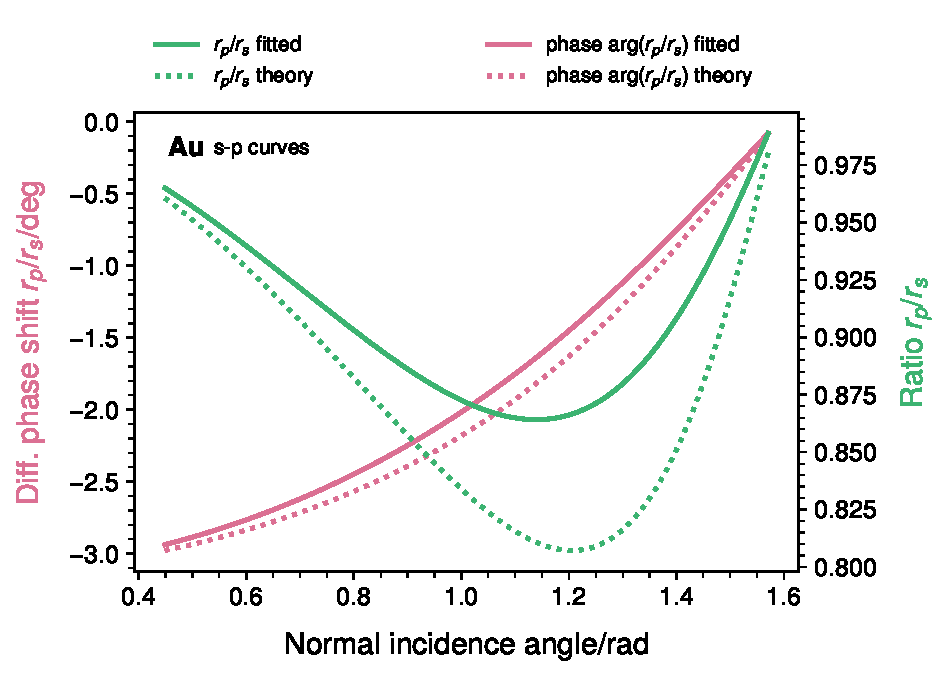
\includegraphics[width=0.45\linewidth]{figures/phase_ratio_Air.Au.pdf}\label{fig:Air.Au.rp/rs}}
    \subfloat[]{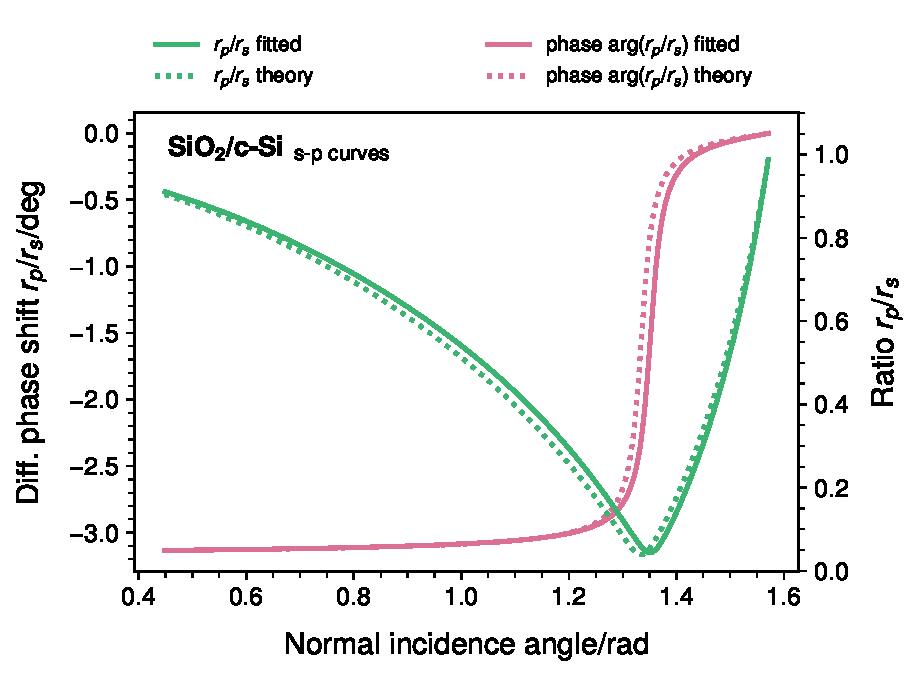
\includegraphics[width=0.45\linewidth]{figures/phase_ratio_Air.SiO2.Si.pdf}\label{fig:Air.SiO2.Si.rp/rs}}
    \caption{\ref{sub@fig:Air.Au.rp/rs}\ref{sub@fig:Air.SiO2.Si.rp/rs}\comment[MS]{Need clear explanation (is actually useful data)}}
    \label{fig:enter-label}
\end{figure*}

\appendix

\bibliography{references/brewster_research}

\end{document}
